% Beamer Presentation and Lecture Note Template
% Version 0.1
% by Paul Vesey

\mode<presentation> {
\usetheme{Antibes}
\setbeamercovered{invisible}
\setbeamertemplate{footline}[frame number]
\setbeamertemplate{navigation symbols}{} 
}

\usepackage{eurosym}
\usepackage{graphicx}
\usepackage{wasysym}
\usepackage{hyperref}
\usepackage{amsmath}
\usepackage{amssymb}
\usepackage{mathtools}
\usepackage{tikz}
\usepackage{pgf}
\usepackage{pgfplots}
\usepackage{pxfonts}
\usepackage{textcomp}
\usepackage{verbatim}
\usepackage{color}
\usepackage{xcolor}
\usepackage{fix-cm}


\author{Paul Vesey}
\institute[TUS]
{
Technological University of the Shannon \\
\medskip
{\emph{paul.vesey@tus.ie}}
}
\date{Autumn 2022}



\title[Project Management \& BIM]{Project Scope Management}
%

\begin{document}
%

\tableofcontents
\newpage



\begin{frame}
\titlepage
\end{frame}\begin{center}\line(1,0){250}\end{center}
%
%


\section{Project Scope Management}

\subsection{Introduction}



\begin{frame}
\frametitle{Scope Management}
Primarily concerned with what is and what is not included in a project.\\
Processes (not in PMBOK order)
\begin{itemize}
 	\item Collect Requirements
 	\item Define Scope
 	\item Verify Scope
 	\item Control Scope
 	\item Create WBS (Work Breakdown Structure)
\end{itemize}
\end{frame}\begin{center}\line(1,0){250}\end{center}



\begin{frame}
\frametitle{A Definition of Scope}
\textbf{\textsc{The work that needs to be accomplished to deliver a product, service or result with the specified features and functions.}}
\end{frame}\begin{center}\line(1,0){250}\end{center}



\begin{frame}
\frametitle{Collect Requirements}{Part of the Planning Process Group}
\begin{figure}
	\centering
		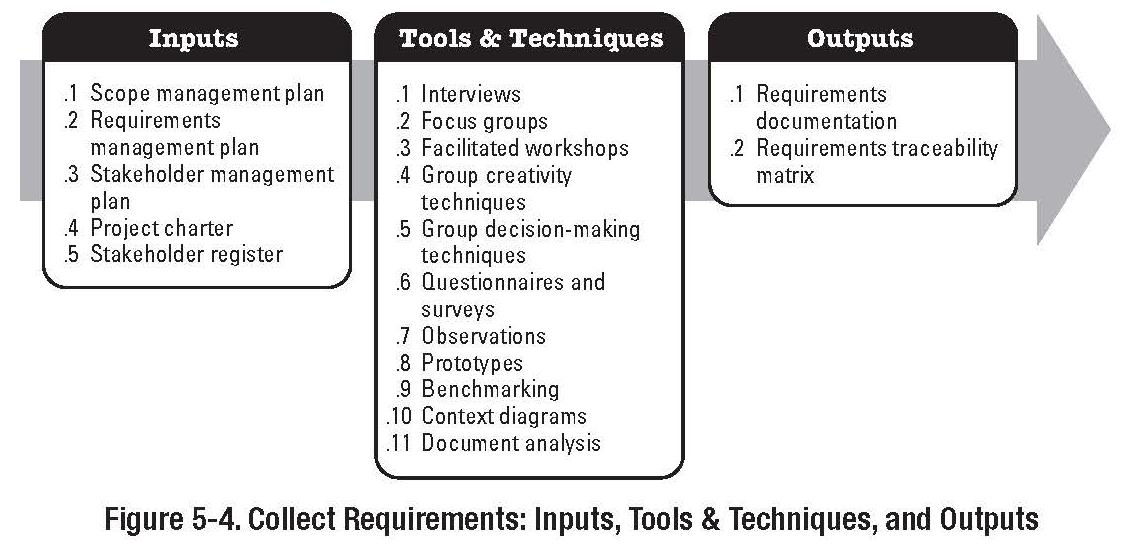
\includegraphics[width = 10cm]{images/Fig5-4.jpg}
	\label{fig:5-4}
\end{figure}
\end{frame}\begin{center}\line(1,0){250}\end{center}



\begin{frame}
\frametitle{Collect Requirements \hfill Tools and Techniques}
Interviews:
\begin{itemize}
	\item Formal or Informal to discover information from Stakeholders
	\item May be one-to-one or one-to-many
\end{itemize}
Focus Groups:
\begin{itemize}
	\item Brings together pre-qualified stakeholders in order to learn about their needs wants and expectations
	\item Trained Moderator leads the discussion
\end{itemize}
\end{frame}\begin{center}\line(1,0){250}\end{center}



\begin{frame}
\frametitle{Collect Requirements \hfill Tools and Techniques}
Facilitated Workshops:
\begin{itemize}
	\item Brings Cross Functional Stakeholders together in a controlled manner
	\begin{itemize}
		\item Build Trust, Improve communications, Increased Stakeholder consensus
	\end{itemize}
\end{itemize}
Group Creativity Techniques:
\begin{itemize}
	\item Brainstorming, Nominal Group Technique, The Delphi Method, Idea/Mind Mapping, Affinity Diagram
\end{itemize}
Refer to book for all
\end{frame}\begin{center}\line(1,0){250}\end{center}



\begin{frame}
\frametitle{Collect Requirements \hfill Tools and Techniques}
Group Decision Making Techniques
\begin{itemize}
	\item Unanimity, Majority, Plurality, Dictatorship
\end{itemize}
Questionnaires and Surveys\\
Observations
\begin{itemize}
	\item Direct Observation (shadowing), Participant Observer
\end{itemize}
Prototypes
\begin{itemize}
	\item Not easy in Construction, perhaps through 3D Design Visualisation Techniques
\end{itemize}
\end{frame}\begin{center}\line(1,0){250}\end{center}



\begin{frame}
\frametitle{Collect Requirements \hfill Outputs}
Requirements Documentation
\begin{itemize}
	\item Refer to Book
	\item Functional Requirements
	\item Non Functional Requirements
	\item Acceptance Criteria
	\item Support and Training Requirements
\end{itemize}
Requirements Management Plan
\begin{itemize}
	\item How changes will be controlled
\end{itemize}
Requirements Traceability Matrix
\begin{itemize}
	\item Links Requirements to project objectives, scope, WBS, Design, etc.
\end{itemize}
\end{frame}\begin{center}\line(1,0){250}\end{center}



\begin{frame}
\frametitle{Define Scope}{Part of the Planning Process Group}
\begin{figure}
	\centering
		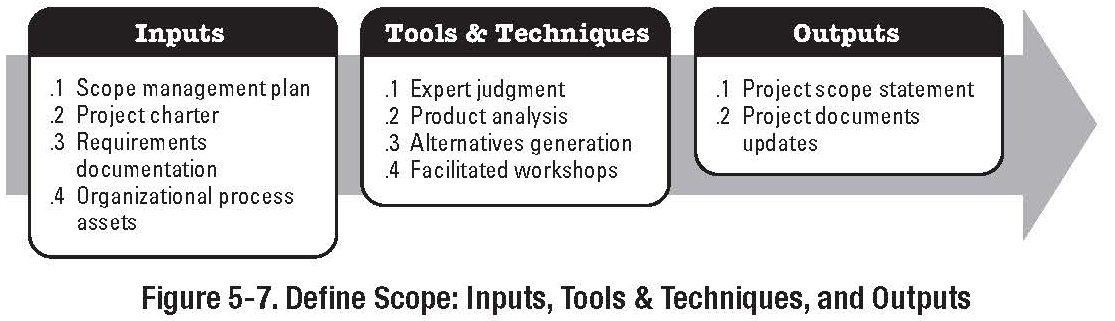
\includegraphics[width = 10cm]{images/Fig5-7.jpg}
	\label{fig:5-7}
\end{figure}
\end{frame}\begin{center}\line(1,0){250}\end{center}



\begin{frame}
\frametitle{Define Scope \hfill Inputs}
Refer to book:
\begin{itemize}
	\item Project Charter
	\item Requirements Documents
	\item Organizational Process Assets
	\item Tools \& Techniques
	\begin{itemize}
		\item Expert Judgment, Product Analysis, Alternatives Identification, Facilitated Workshops
	\end{itemize}
\end{itemize}
\end{frame}\begin{center}\line(1,0){250}\end{center}



\begin{frame}
\frametitle{Define Scope}
Product Analysis:
\begin{itemize}
	\item  It is a method of converting product descriptions (drawings, specs, etc.) and project objectives (build times, build costs) into deliverables and requirements.
	\item Included Techniques such as product breakdown, systems analysis, system engineering, value engineering, value analysis, and functional analysis
\end{itemize}
\end{frame}\begin{center}\line(1,0){250}\end{center}



\begin{frame}
\frametitle{Define Scope \hfill Stakeholder Analysis}
\begin{itemize}
	\item Identifying Stakeholders
	\item Understanding Stakeholder Roles
	\begin{itemize}
		\item Interests, objectives, influence
	\end{itemize}
	\item Communicating with Stakeholders
	\begin{itemize}
		\item	Determine needs, wants, expectations
		\item	Separate `key requirements' from `wish lists'
		\item Alternatives Identification
	\end{itemize}
	\item Technique to discover alternative methods and ways of accomplishing the project.
	\begin{itemize}
		\item Brainstorming
		\item Lateral thinking
	\end{itemize}
\end{itemize}
\end{frame}\begin{center}\line(1,0){250}\end{center}



\begin{frame}
\frametitle{Define Scope \hfill Alternatives Identification}
Technique to discover alternative methods and ways of accomplishing the project.
\begin{itemize}
	\item Brainstorming, Lateral thinking, Facilitated Workshops
\end{itemize}
Involve Stakeholders
\begin{itemize}
	\item Make sure you understand Stakeholder's Roles
	\item Interests, objectives, influence
	\item As a facilitator; Determine needs, wants, expectations, Separate `key requirements' from `wish lists'
\end{itemize}
\end{frame}\begin{center}\line(1,0){250}\end{center}



\begin{frame}
\frametitle{Scope Definition \hfill Output}
Project Scope Statement, which includes:\\ 
(refer to book for details) 

\begin{table}
\scalebox{0.8}{
	\centering
		\begin{tabular}{|c|l|c|l|}
		\hline
			1 & 	Project Objectives 			& 	9	& 	Initial Project Organisation \\
			2	& 	Product Scope Description 	& 	10	& 	Initial Identified Risks \\
			3	& 	Project Requirements 		& 	11	& 	Schedule Milestones \\
			4	& 	Project Boundaries 			& 	12	& 	Fund Limitations \\
			5	& 	Project Deliverables 		& 	13	& 	Cost Estimate \\
			6	& 	Product Acceptance Criteria & 	14	& 	Config MGMT Requirements \\
			7	& 	Project Constraints 		& 	15	&   Project Specifications \\
			8	& 	Project Assumptions 		& 	16	& 	Approval Requirements \\
		\hline
		\end{tabular}
	\label{tbl:elements}
}	
\end{table}

\end{frame}\begin{center}\line(1,0){250}\end{center}



\begin{frame}
\frametitle{Define Scope}
Project Objectives should be SMART
\begin{itemize}
	\item \textbf{S}pecific
	\item \textbf{M}easurable
	\item \textbf{A}ccurate
	\item \textbf{R}ealistic and Tangible
	\item \textbf{T}ime Bound
\end{itemize}
Project Deliverables  
\begin{itemize}
	\item measurable outcomes, measurable results, and specific items that must be produced to consider the project (or project phase) complete. 
\end{itemize}
\end{frame}\begin{center}\line(1,0){250}\end{center}



\begin{frame}
\frametitle{Define Scope}
Project Acceptance Criteria
\begin{itemize}
	\item Processes (tests) and criteria for acceptance by the client.
		\begin{itemize}
			\item i.e. WT plant, producing 10 MLD of potable water compliant with EU regs.
		\end{itemize}
\end{itemize}
Project Constraints
\begin{itemize}
	\item Time constraints
	\item Budget constraints
	\item Quality constraints
	\item Schedule constraints
	\item Technology constraints
\end{itemize}
\end{frame}\begin{center}\line(1,0){250}\end{center}



\begin{frame}
\frametitle{Project Assumptions}
\emph{When you `assume' you make an `ass' out of `u' and `me'}\smiley{}\\
You can't know everything, so you will have to make assumptions.\\
\textbf{For PM, it is vital that you record all assumptions and get the project sponsor to sign off on those assumptions}\\
\begin{itemize}
	\item Typical internal assumptions would be the availability of key personnel and/or equipment for a project
	\item Typical external assumptions would be that the client (sponsor) will have necessary all planning permissions.
\end{itemize}
\end{frame}\begin{center}\line(1,0){250}\end{center}



\begin{frame}
\frametitle{Scope Statement}
\begin{itemize}
	\item Provides the basis for making future decisions in relation to scope changes
	\item Intended to make sure that all stakeholders have a common knowledge of what the project entails
	\item Addresses 7 key questions:
	\begin{itemize}
		\item Who, What, When, Why, Where, How, How many
	\end{itemize}
\end{itemize}
\begin{block}{The Elephants Child - Rudyard Kipling (1902)}
I keep 6 honest serving men,\\
	\hspace{2cm}(they taught me all I knew),\\
Their names are What and Why and When,\\
	\hspace{2cm} And How and Where and Who.\\
\end{block}
\end{frame}\begin{center}\line(1,0){250}\end{center}



\begin{frame}
\frametitle{Scope Statement v. Statement of Work (SOW)}
\begin{itemize}
	\item Scope Statement is generated by the PM team
	\item Statement of Work is generated by the client
	\item Statement of Work is a narrative description of the end results to be provided under the contract
\end{itemize}
For construction contracts, the SOW typically provides the basis for the Scope Statement
\end{frame}\begin{center}\line(1,0){250}\end{center}



\begin{frame}
\frametitle{Scope Statement and SOW}
Both the client and the contractor must `sign-off' on the Scope Statement and SOW.
\begin{itemize}
	\item SOW is normally written into the contract and therefore signed off on.
\end{itemize}
An order of priority must also be agreed.
\begin{itemize}
	\item i.e. SOW is typically given priority over the Scope Statement.  If a discrepancy arises between the documents the SOW will be upheld.
\end{itemize}
\end{frame}\begin{center}\line(1,0){250}\end{center}



\begin{frame}
\frametitle{Misinterpretation \hfill Common Causes}
\begin{itemize}
	\item Mixing tasks, specifications, approvals, and special instructions
	\item Using imprecise language
	\begin{itemize}
		\item `nearly' `optimum', `approximately', etc.
	\end{itemize}	
	\item No pattern, structure or chronological order
	\item Wide variation in size of tasks
	\item Wide variation in how to describe details of work
	\item Failing to obtain third-party review
\end{itemize}
\end{frame}\begin{center}\line(1,0){250}\end{center}



\begin{frame}
\frametitle{Misinterpretation \hfill Fixes}
In an effort to avoid pitfalls a number of private and public bodies have issued guidelines for the preparation of Scope Statements and SOWs\\
NASA SOW Guidance Available from: \href{http://www.hq.nasa.gov/office/procurement/newreq1.htm}{www.hq.nasa.gov/office/procurement/newreq1.htm}
\end{frame}\begin{center}\line(1,0){250}\end{center}



\begin{frame}
\frametitle{Advantages of Scope Statements}
\begin{itemize}
	\item Enables client and contractor to understand the project requirements and needs.
	\item Reduces claims and disputes under the contract by identifying potential issues early in the project.
	\item Forces Designers, Engineers, PM team, QS team, CM team, etc. to re-examine the SOW in detail. 
		\begin{itemize}
			\item (typically post tender, and pre-contract signing)
		\end{itemize}
	\item Minimises RFIs and Change Orders; and the delays associated.
	\item Provides a clear baseline for performance that covers the virtually every aspect of the project.
	\item Clarifies acceptance tests and criteria early in the project.
\end{itemize}
\end{frame}\begin{center}\line(1,0){250}\end{center}



\begin{frame}
\frametitle{Validate Scope}{Part of the Monitoring \& Controlling Process Group}
\begin{figure}
	\centering
		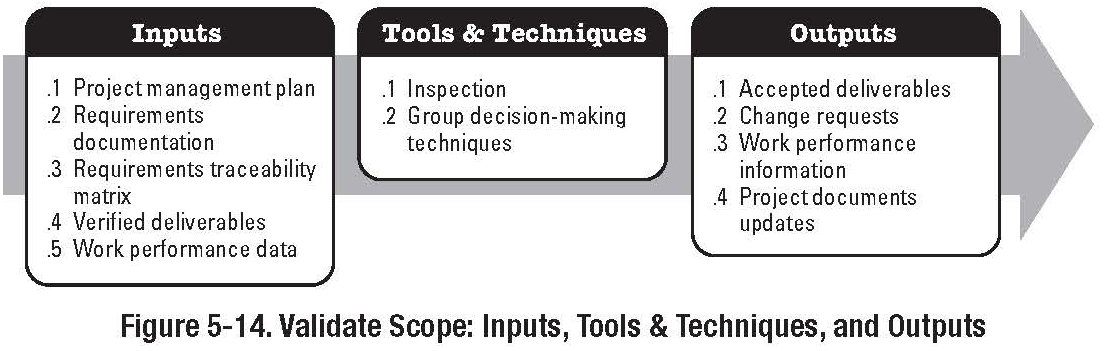
\includegraphics[width = 10cm]{images/Fig5-14.jpg}
	\label{fig:Fig5-14}
\end{figure}
\end{frame}\begin{center}\line(1,0){250}\end{center}



\begin{frame}
\frametitle{Scope Validation}
\begin{itemize}
	\item Scope Validation is carried out over the entire project duration, not just at the start
	\item Initial Validation involves obtaining the stakeholders formal acceptance of the project scope and associated deliverables.
	\begin{itemize}
		\item This first Scope Statement is referred to as the \textbf{`Baseline Scope Statement'}
	\end{itemize}
	\item Thereafter, Scope Validation is involved with checking and verifying that project deliverables and requirements are being met in accordance with the Scope Statement
\end{itemize}
\end{frame}\begin{center}\line(1,0){250}\end{center}



\begin{frame}
\frametitle{Scope Validation \hfill Cont\ldots}
\begin{itemize}
	\item Validation includes inspections to ensure that Project Deliverables are being met and accepted.
	\item If Project Deliverables are not being accepted, the validation process records the reasons for rejection.
	\item Rejection typically leads to Requested Changes, which are passed to the Integrated Change Control Process to identify potential impacts on time, cost, etc.
	\item Rejection can also lead to Corrective Actions (ie Rework)
\end{itemize}
\end{frame}\begin{center}\line(1,0){250}\end{center}

\subsection{Scope Control}

\begin{frame}
\frametitle{Control Scope}{Part of the Monitoring and Controlling Process Group}
\begin{figure}
	\centering
		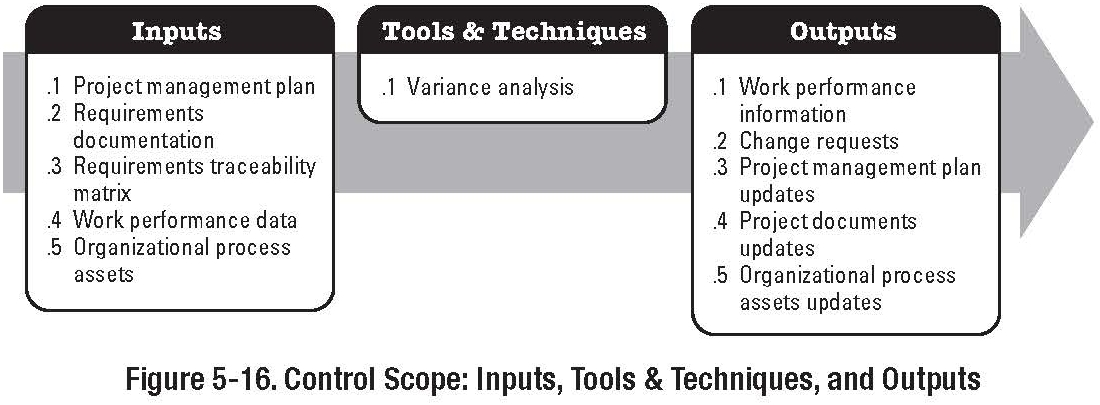
\includegraphics[width = 10cm]{images/Fig5-16.jpg}
	\label{fig:5-16}
\end{figure}
\end{frame}\begin{center}\line(1,0){250}\end{center}



\begin{frame}
\frametitle{Control Scope}
Scope Creep\ldots
\emph{There is no such thing as scope creep, only scope gallop} \smiley{}\\
AKA `kitchen sink syndrome' \smiley{}\\
\begin{itemize}
	\item It is a gradual process, by which additional (unauthorized) work is added to the original project 
	\item If not properly handled, it can destroy a project and a Project Manager's reputation.
\end{itemize}
\end{frame}\begin{center}\line(1,0){250}\end{center}



\begin{frame}
\frametitle{Scope Creep}
Provided it is controlled, it is not always a bad thing
\begin{itemize}
	\item Can lead to increased profitability of a contract
\end{itemize}
Sometimes used by the unscrupulous as  a means to bargain for an EOT to a contract
\begin{itemize}
	\item Additional works anticipated to take 2 weeks
	\item propose to carry out the works on condition that an EOT of 3 weeks is granted.
	\item New DoF Contracts make this very difficult
\end{itemize}
\end{frame}\begin{center}\line(1,0){250}\end{center}



\begin{frame}
\frametitle{Control Scope}
Inputs:
\begin{itemize}
	\item Partially covered; refer to book
\end{itemize}
Outputs (refer to book for details)
\begin{itemize}
	\item Work Performance Measurements
	\item Organisational Process Assets Updates
	\item Change Requests - Scope control does not mean always saying `no'
	\item Project Management Plan Updates
		\begin{itemize}
			\item Scope Baseline Update
			\item Other Baseline Updates (Time, Cost, etc.)
		\end{itemize}
	\item Project Document Updates - Requirements Documents, etc.
\end{itemize}
\end{frame}\begin{center}\line(1,0){250}\end{center}



\begin{frame}
\frametitle{Control Scope \hfill Tools and Techniques}
Variance Analysis:
\begin{itemize}
	\item Determination of the magnitude of variations
	\item Determination of the cause of variations
		\begin{itemize}
			\item Some variations are borne by the client; others by the contractor
		\end{itemize}
	\item Re-planning
		\begin{itemize}
			\item Approved change requests can effect the project scope usually require changes to the WBS, WBS dictionary, Schedules, Scope Statement, PM Plan etc.
		\end{itemize}
	\item Change Control System
		\begin{itemize}
			\item Impact assessment, documentation, authorization, etc.
		\end{itemize}
\end{itemize}
\end{frame}\begin{center}\line(1,0){250}\end{center}




\subsection{Work Breakdown Structure}


\begin{frame}
\frametitle{Create Work Breakdown Structure}{Part of the Planning Process Group}
\begin{figure}
	\centering
		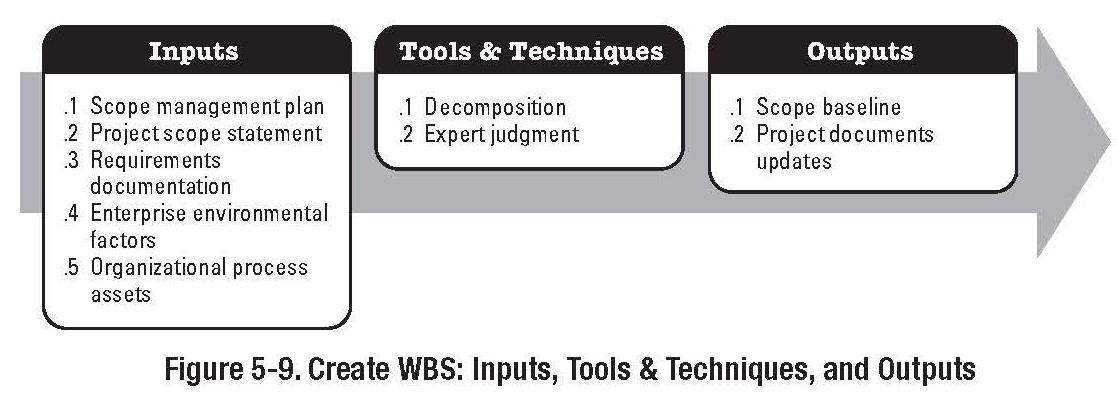
\includegraphics[width = 10cm]{images/Fig5-9.jpg}
	\label{fig:5-9}
\end{figure}
\end{frame}\begin{center}\line(1,0){250}\end{center}



\begin{frame}
\frametitle{Work Breakdown Structure}
\emph{A hierarchical decomposition of the total scope of work to be carried out by the project team to accomplish project objectives and create the required deliverables.}\\
\hspace{2cm} PMBOK\textregistered definition.. P567
\end{frame}\begin{center}\line(1,0){250}\end{center}



\begin{frame}
\frametitle{Work Breakdown Structure}
The importance of the WBS cannot be over emphasized\\
Failure to develop a sufficiently detailed WBS will lead to:\\
\begin{itemize}
	\item Scheduling issues
	\item Procurement issues
	\item Costing and Budgeting issues
	\item Status Reporting issues
	\item Unclear delegation of responsibilities
	\item Etc.
\end{itemize}
\end{frame}\begin{center}\line(1,0){250}\end{center}



\begin{frame}
\frametitle{}
\begin{figure}
	\centering
		\includegraphics[width = 10cm]{images/fig5-11.jpg}
	\label{fig:5-11}
\end{figure}
\end{frame}\begin{center}\line(1,0){250}\end{center}




\begin{frame}
\frametitle{}
\begin{figure}
	\centering
		\includegraphics[width = 10cm]{images/fig5-12.jpg}
	\label{fig:5-12}
\end{figure}
\end{frame}\begin{center}\line(1,0){250}\end{center}




\begin{frame}
\frametitle{}
\begin{figure}
	\centering
		\includegraphics[width = 10cm]{images/fig5-13.jpg}
	\label{fig:5-13}
\end{figure}
\end{frame}\begin{center}\line(1,0){250}\end{center}








\begin{frame}
\frametitle{Sample WBS}
\begin{figure}
	\centering
		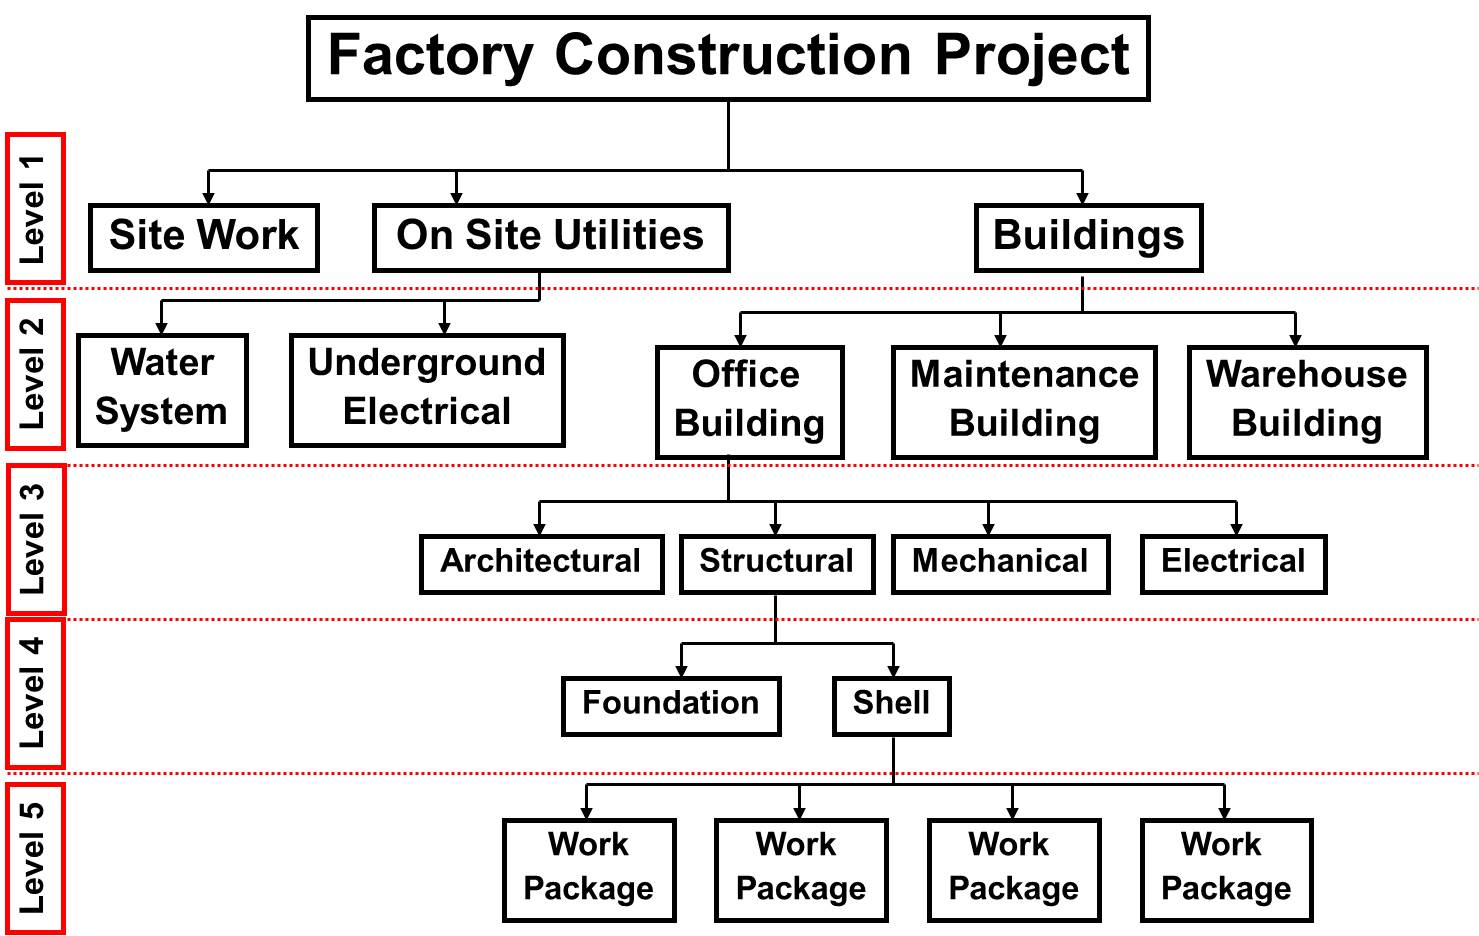
\includegraphics[width = 10cm]{images/wbs.jpg}
	\label{fig:wbs}
\end{figure}
\end{frame}\begin{center}\line(1,0){250}\end{center}



\begin{frame}
\frametitle{Sample WBS with Numbering Scheme}
\begin{figure}
	\centering
		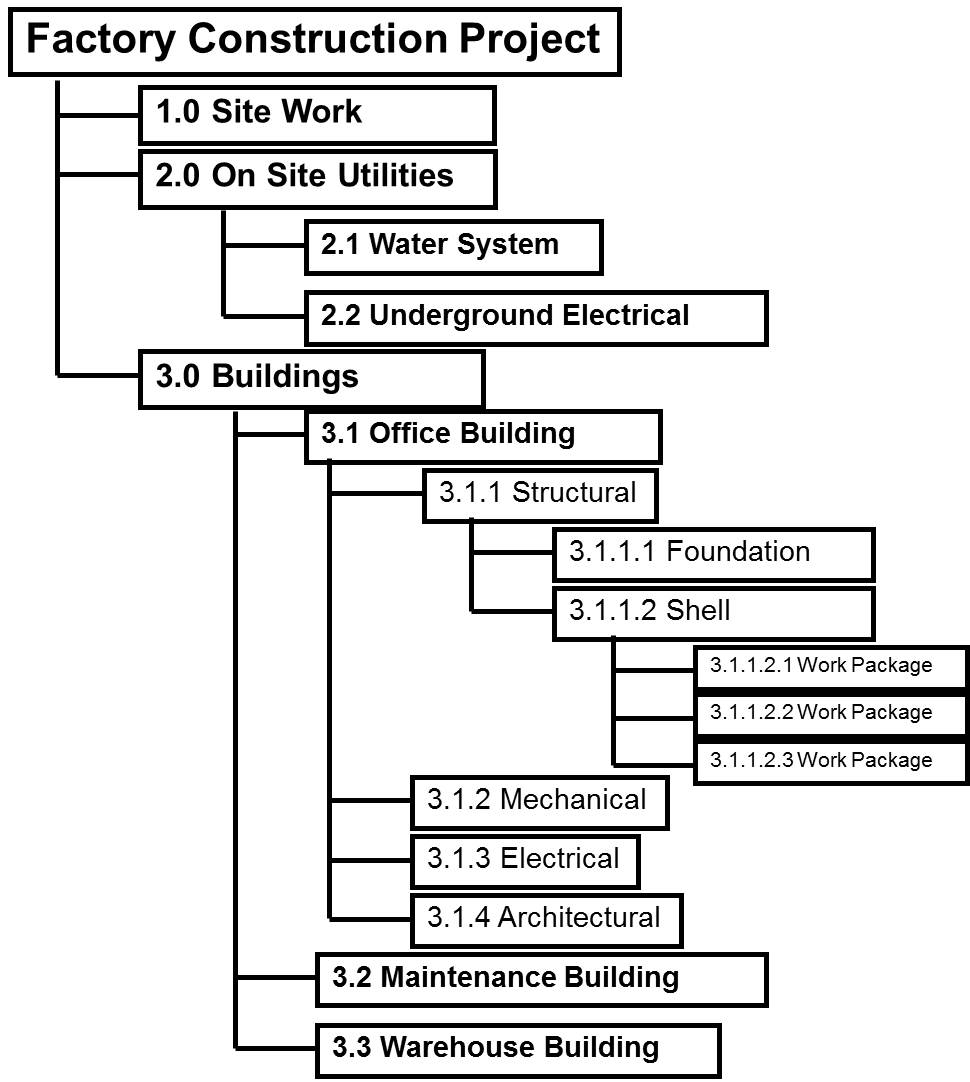
\includegraphics[width = 5cm]{images/wbscode.jpg}
	\label{fig:wbscode}
\end{figure}
\end{frame}\begin{center}\line(1,0){250}\end{center}



\begin{frame}
\frametitle{MS Project}
\begin{figure}
	\centering
		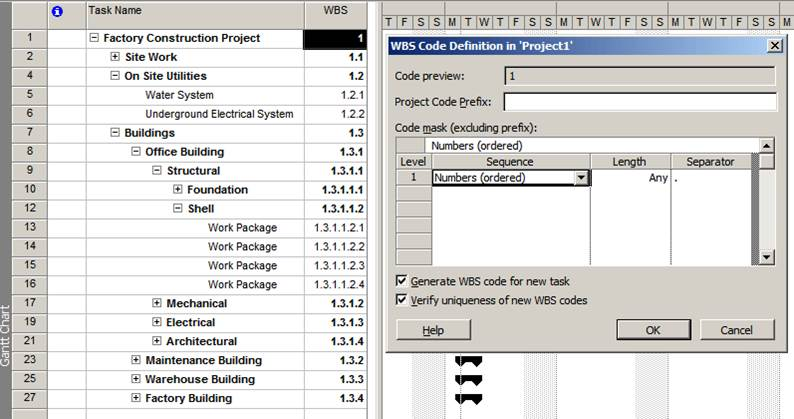
\includegraphics[width = 10cm]{images/msprojectwbs.jpg}
	\label{fig:msprojectwbs}
\end{figure}
MS Project has WBS code functionality included\\ 
use Project | WBS | Define Code
\end{frame}\begin{center}\line(1,0){250}\end{center}



\begin{frame}
\frametitle{WBS Levels}
Dependant upon project, but in general:\\
\begin{itemize}
	\item Level 1 - Total Program
	\item Level 2 - Project 
	\item Level 3 - Task
	\item Level 4 - Subtask
	\item Level 5 - Work Package
	\item Level 6 - Level of Effort
\end{itemize}
Managerial Levels - 1 to 3 (Project Manager)\\
Technical Levels - 4 to 6 (Line Managers)\\
\end{frame}\begin{center}\line(1,0){250}\end{center}



\begin{frame}
\frametitle{}
When the project (and work to be completed) is organised in this way it provides a framework for:
\begin{itemize}
	\item Planning to be performed
	\item Costs and Budgets to be established
	\item Time, cost and performance to be tracked
	\item Schedules and Status reporting procedures to be established
	\item Responsibility for delivery of elements to be established and tracked
	\item Risk Analysis
	\item Development of an Organisation Structure and Responsibility Matrix
\end{itemize}
By breaking down the overall project into its constituent elements, the probability that every major and minor component will be completed is increased.
\end{frame}\begin{center}\line(1,0){250}\end{center}



\begin{frame}
\frametitle{More on Levels\ldots}
The upper 3 levels of the WBS are usually specified by the customer (SOW)
\begin{itemize}
	\item Level 1 is generally used for authorization and release of all work
	\item Level 2 is generally used for budget preparation
	\item Level 3 is generally used for schedule preparation
\end{itemize}
The lower 3 levels are generated by the contractor for in-house control
\end{frame}\begin{center}\line(1,0){250}\end{center}



\begin{frame}
\frametitle{Considerations when Generating a WBS}
\begin{enumerate}
	\item The WBS and work description should be easy to understand
	\item All schedules should follow the WBS, not the other way around
	\item Work should not be subdivided to the lowest possible level - it is inefficient
	\item The WBS normally changes over the course of a project; build in flexibility
	\item The WBS can act as a list of milestones that can be used to assist communication project progress
	\item The WBS can be used to segregate recurring from non-recurring costs
	\item Most WBS elements range from 0.5\% to 2.5\% of the total project budget - 200 to 40 items
\end{enumerate}
\end{frame}\begin{center}\line(1,0){250}\end{center}



\begin{frame}
\frametitle{WBS tasks and sub-tasks}
WBS tasks should:
\begin{itemize}
	\item Have clearly defined start and end dates
	\item Be usable as a communications tool in which results can be compared with expectations
	\item Be estimated on a `total' time duration, not when a task should start and end 
		\begin{itemize}
			\item Necessary for correct scheduling and network analysis
		\end{itemize}
\end{itemize}
\end{frame}\begin{center}\line(1,0){250}\end{center}



\begin{frame}
\frametitle{Work Packages}
Characteristics:
\begin{itemize}
	\item Represents the units of work at the level where the work is performed
	\item Clearly distinguishes one work package from all others assigned to a functional group
	\item Contains clearly defined start and end dates that are representative of physical accomplishment (done after scheduling)
	\item Specifies a budget in terms of money (\euro), man-hours, or other measurable units
	\item Limits work to be performed to relatively short periods of time.
\end{itemize}
\textbf{Minimises Work in Progress}
\end{frame}\begin{center}\line(1,0){250}\end{center}



\begin{frame}
\frametitle{Example Work Package}
\begin{figure}
	\centering
		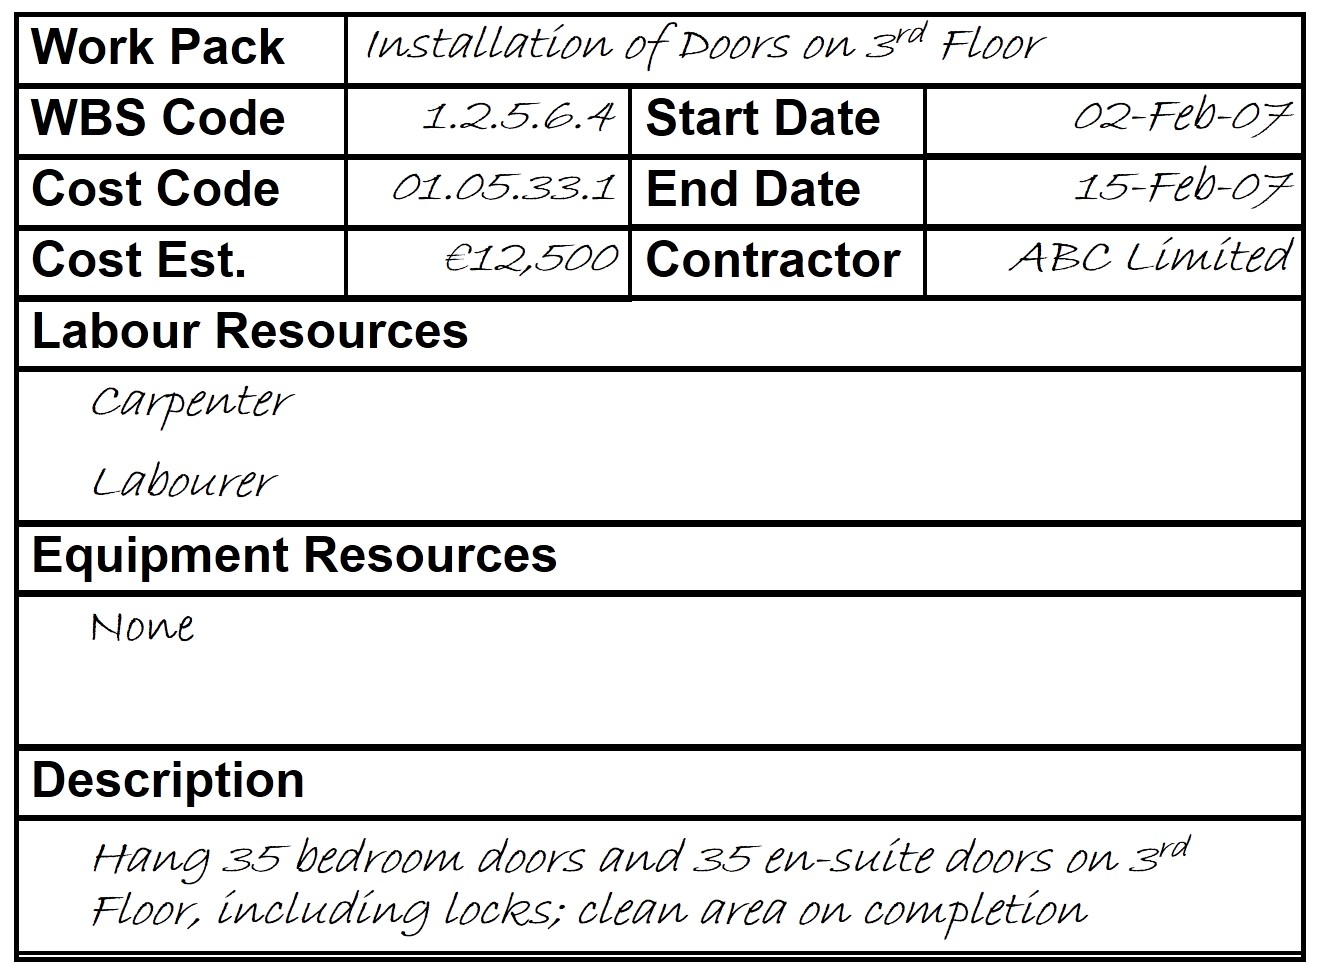
\includegraphics[width = 8cm]{images/pheader.jpg}
	\label{fig:pheader}
\end{figure}
\end{frame}\begin{center}\line(1,0){250}\end{center}



\begin{frame}
\frametitle{WBS Dictionary}
The WBS dictionary is a companion document to the WBS\\
The WBS dictionary describes the WBS elements in terms of:
\begin{itemize}
	\item Account Code identifier
	\item Description of work \& resources required
	\item Organisation responsible
	\item Milestones
	\item Contractual Information
	\item Quality Requirements
	\item Associated schedule activities
	\item Estimate of Cost
	\item See Work Package Header
\end{itemize}
\end{frame}\begin{center}\line(1,0){250}\end{center}



\begin{frame}
\frametitle{WBS Checklist}
\begin{itemize}
	\item Check the WBS for 
	\begin{itemize}
		\item Completeness 
		\item Anticipated effort (time \& resources)
		\item Compatibility
		\item Continuity
	\end{itemize}
	\item Ensure it satisfies both functional and project requirements
	\item Check that the WBS provides a logical subdivisions of project work
	\item Ensure that elements can be assigned to specific individuals and/or groups
	\item Check the WBS against project reporting requirements
\end{itemize}

\end{frame}\begin{center}\line(1,0){250}\end{center}



\begin{frame}
\frametitle{WBS for Sub-Contracting}
\begin{itemize}
	\item Develop a preliminary WBS for top 3 levels
	\item Ensure the Sub-contractor develops the WBS for all lower levels, and submits this information as part of their proposal and reaffirms as part of the sub-contract.
	\item Ensure that the Sub-contractors WBS is compatible with project reporting requirements and the SC's own reporting and management procedures
	\item In short, a Sub-Contractors WBS should be capable of full integration into the project WBS, including elements such as
	\begin{itemize}
		\item Cost, Schedule, Resources, etc.
	\end{itemize}
\end{itemize}
\end{frame}\begin{center}\line(1,0){250}\end{center}



\begin{frame}
\frametitle{WBS Decomposition Problems}
\begin{itemize}
	\item Whilst Levels 1 to 3 can be fairly standard for most construction projects, Levels 4 to 6 can be very difficult to generate
	\item Breaking down work to small and detailed packages may require the creation of hundreds of cost accounts and charge numbers
	\item The costs associated with producing detailed work packages may outweigh the benefits
	\item The WBS forms the basis of Arrow Diagrams and Precedence Diagrams.  At low levels of the WBS, the number of interconnections and dependencies over complicate the network, and can render it impossible to interpret.
\end{itemize}
\end{frame}\begin{center}\line(1,0){250}\end{center}



\begin{frame}
\frametitle{WBS Standardisation}
\begin{itemize}
	\item Many companies who execute projects of similar nature will standardise the top 3 levels of the WBS.
	\item By standardising the top levels of the WBS organisations can compare previous projects, deliverables, costing, execution etc.
	\item Standardisation also lessens the time taken to develop detailed WBS
	\item Standardisation aids communications, and facilitates the transfer of resources and equipment between projects.
\end{itemize}
\end{frame}\begin{center}\line(1,0){250}\end{center}



\begin{frame}
\frametitle{WBS Process Outputs}
\begin{itemize}
	\item WBS
	\item WBS Dictionary
	\item Scope Baseline
	\item Project Document Updates
\end{itemize}
Typically during the generation and review of the WBS previously unidentified elements arise.  These may need to be incorporated into the project, and therefore the Project Scope, and Work Breakdown Structure may require updating through the Integrated Change Control Process
\end{frame}\begin{center}\line(1,0){250}\end{center}



% End of slides
\end{document} 